%Preambolo per documento generico
%Per cambiare tipo di documento modificare
%il documentclass.

\documentclass[11pt]{article}
\usepackage[utf8]{inputenc}

%Mettere italian se si vuole scrivere in italiano
\usepackage[english]{babel}


%Aumento dell'interlinea
\usepackage{setspace}
\onehalfspacing

%Pacchetti per simboli matematici
\usepackage{mathtools}
\usepackage{amsfonts}
\usepackage{amsthm}
\newtheorem{theorem}{Theorem}
\usepackage{amsmath}
\usepackage{bm}

\usepackage[dvipsnames]{xcolor}
\definecolor{sapred}{RGB}{130,36,51} %colore sapienza per i titoli


%Pacchetti per figure e tabelle
\usepackage{booktabs, caption, graphicx, subfig, float}
\captionsetup{tableposition=top,figureposition=bottom,font=small}

%Per inserire commenti in blocco
%Usage: \begin{comment} ... \end{comment}
\usepackage{comment}

%Definisce colori dei link nel testo e altri parametri
\usepackage{hyperref}
\hypersetup{
pdftitle={Rendez-vous and formation control for unicycles via consensus},%
pdfauthor={SDF,AT,AW},%
pdfsubject={Multi Robot},%
pdfkeywords={},%
colorlinks=true,%
linkcolor=black,%
linktocpage=true,%
pageanchor=true,
citecolor=black
}

%Definisce in maniera simmetrica i margini di pagina
\usepackage{geometry}
\geometry{a4paper, top=3cm,bottom=3cm,left=3cm,right=3cm,%
			heightrounded}

%Per scrivere in maniera rapida norme e valori assoluti
%Usage: y = \abs{x} ; y = \norma{x}
\DeclarePairedDelimiter{\abs}{\lvert}{\rvert}
\DeclarePairedDelimiter{\norma}{\lVert}{\rVert}

%Testo a caso
%Usage: \lipsum[a-b] | Esempio \lipsum[1-10]
\usepackage{lipsum}

%Cambia lo stile della pagina
%In alto a dx mette numero di pagina
%In alto a sinistra titolo e autore
\usepackage{fancyhdr}
\pagestyle{fancy}
\fancyhf{}
\rhead{\textit{\thepage}}
\lhead{\textit{Rendez-vous and formation control for unicycles via consensus}}

%Per inserire codice nativo MATLAB e simili
%Usage: guardare sotto
\usepackage{fancyvrb}




\begin{document}

\title{\textbf{\textcolor{sapred}{Rendez-vous and formation control for unicycles via consensus}}}
\author{Stefano De Filippis \\
Andrea Tantucci \\
Andrea Wrona}
%Optional: data. Se non si inserisce il campo data
%LaTeX mette la data del PC automaticamente
%\date{}
\maketitle

\thispagestyle{empty}

\section*{Theoretical Background}
The aim of this project is the study and implementation of a controller that solves the consensus problem in case of a network of nonlinear systems. The single system that will be used is the unicycle and in the following sections, after an introduction about the problem to be solved, a nonlinear controller will be designed and also a stability analysis will be conducted to prove the convergence of the control law.

Eventually, the experiments results will be reported considering different case scenarios where the number of interconnected agents is continuously increased in the settings and also slightly modifying parameters in order to show some feasibility issues that can arise with the proposed control law.

\subsection*{Rendzevous Problem}

The Rendzevous problem can be seen as a specific application of the theoretical problem represented by the Consensus problem. In the case of the Consensus Protocol the problem can be formulated by considering $N$ agents with an internal state $x_i \in \mathbb{R}$ , each with an internal dynamics for the state evolution $\dot{x}_i = f_i(x_i,u_i)$. Moreover, the agents are interconnected and this information is encoded through an interaction graph $G$ that has the agents as vertexes and the edges representing the information flow.

Therefore, the problem is to design control inputs $u_i$ so that all the states $x_i$ converge to the same unspecified common value $\bar{x}$

\begin{equation}
\lim_{t\rightarrow\infty}x_i(t) = \bar{x}, \quad \forall i
\end{equation}
considering that in the control $u_i$ only relative information represented by the information flow can be used.
If we have $N$ identical mobile robots, whose state $x_i$ is represented by the position on the plane and its orientation, then the rendezvous problem consists in moving all the robots to a common location with the same orientation.

\subsection*{Consensus Protocol}

If the single system in the network is represent by a single integrator $\dot{x_i} = u_i$, the control can be simply defined as the sum of all the differences of the neighbors' states w.r.t. the state of agent $i$

\begin{equation}
u_i = \sum_{j \in \mathcal{N}_i}(x_j - x_i) = -Lx
\end{equation}
where $L$ is the Laplacian of the interaction graph and $x$ is the concatenation of all the states.

It can be proven that if $G$ is connected then the consensus problem is actually solved and it is

\begin{equation}
\lim_{t\rightarrow\infty} x = \frac{(\mathbf{1}^Tx_0)\mathbf{1}}{N}
\end{equation}
which means that each state converges to the average of the initial state.

If we consider a system whose dynamics is nonlinear, though, this control law cannot be directly applied and so a new controller needs to be designed. This new control law will somehow extend this simple approach just described and it will still rely only on relative information and will be a function of the relative differences of the neighbors' states.

\subsection*{Unicycle Model}

In particular, in the case study the agents considered are unicycles. The dynamics of this system is derived at a kinematic level by considering the nonholonomic motion constraint that arises due to the pure rolling constraint.

The state of the system is given by the position on the plane and its orientation $(x, y, \theta)$ and at each instant the agent is only allowed to move along its saggital axis. The resulting system is

\begin{align}
&\dot{x} = u\cos\theta\\
&\dot{y} = u\sin\theta\\
&\dot{\theta} = \omega.
\end{align}
The controls $(u, \theta)$ can be designed and interpreted as the velocity and angular velocity of the unicycle.

\subsection*{Potential Forces}

The general approach that will be used in order to derive a suitable control law makes use of potential forces, which present the form

\begin{equation}
f(z) = -z[f_a(||z||)-f_r(||z||)]
\end{equation}
where $f_a: \mathbb{R}^+ \rightarrow \mathbb{R}^+$ is the magnitude of an attraction term, $f_r: \mathbb{R}^+ \rightarrow \mathbb{R}^+$ is the magnitude of a repulsive term and $||z|| = \sqrt{z^Tz}$ is the euclidean norm.

There exists a unique constant distance $\delta$ where the two forces exactly balance $f_a(\delta) = f_r(\delta)$, while $f_a(||z||) > f_r(||z||)$ holds $\forall||z|| > \delta$, and $f_a(||z||) < f_r(||z||)$ holds $\forall||z|| < \delta$.

Note that $-zf_a(||z||)$ represents the actual attraction force, whereas $zf_r(||z||)$ represents tye actual repulsion and they both act along the line connecting the two agents which is represented by $z$.

\subsection*{Control Law for Rendezvous Problem}

In this section, the control law in order to solve the rendezvous problem is defined.

Consider $n$ agents scattered in a plane with random orientations. The agents exchange information comprising the position of the neighboring agents whose interconnection is defined by a graph $G$ that needs to be balanced and (strongly) connected.

In order to make the headings converge, the angular velocity command is defined as:

\begin{equation}
\omega_i = -\sum_{j \in \mathcal{N}_i} (\theta_i - \phi_{ij})
\end{equation}
with
\begin{equation}
\phi_{ij} = \arctan\begin{pmatrix}
\frac{y_j-y_i}{x_j-x_i}
\end{pmatrix}
\end{equation}
which lets the heading of agent $i$ point into the direction of the agents in its neighborhood $\mathcal{N}_i$. Then, in order to make the agents meet at a point the attractive potential function can be considered

\begin{equation}
g_a(||d_i||) = \frac{1}{2}||d_i||^2 = \frac{1}{2}d_i^Td_i
\end{equation}
with
\begin{equation}
d_i = \begin{pmatrix}
x_i - x_i\\
y_i - y_j
\end{pmatrix}
\end{equation}

Then, the consensus can be achieved defining

\begin{align}
& u_i = -\sum_{j \in \mathcal{N}_i} \nabla g_a^Tt_i = -\sum_{j \in \mathcal{N}_i} [(x_i - x_j)\cos\theta_i + (y_i - y_j)\sin\theta_i]\\
& \omega_i = -\sum_{j \in \mathcal{N}_i} (\theta_i - \phi_{ij})
\end{align}
where $t_i$ represents the unit heading vector of agent $i$.

It is important to notice that while adjusting their headings w.r.t. the neighboring agents, all the agents approach each other such that the velocity $u_i \rightarrow 0$ as the agents converge to the same location. Thus, the equilibrium for the aggregate system is $d_{i,e} = 0$ and $\theta_{i,e} = \phi_{i,j}$. 

\subsection*{Stability Analysis}

In this section the stability of the aggregate system consisting of $n$ copies of the single unicycle with the rendezvous controller will be tackled and which results in the dynamics

\begin{align*}
&\dot{d}_i = -\sum_{j \in \mathcal{N}_i}H_id_i\\
&\dot{\theta}_i = -\sum_{j \in \mathcal{N}_i} \begin{bmatrix}\theta_i - \arctan\begin{pmatrix}
\frac{y_j-y_i}{x_j-x_i}
\end{pmatrix}\end{bmatrix}
\end{align*}
where

\begin{equation}
H_i = \begin{pmatrix}
\cos^2\theta_i+\cos^2\theta_j & \cos\theta_i\sin\theta_i+\cos\theta_j\sin\theta_j\\
\cos\theta_i\sin\theta_i+\cos\theta_i+\cos\theta_j\sin\theta_j & \sin^2\theta_i+\sin^2\theta_j
\end{pmatrix}
\end{equation}

As Lyapunov candidate the following function is considered

\begin{equation}
V = \sum_{i = 1}^nV_i = \sum_{i = 1}^n\sum_{j \in \mathcal{N}_i}\frac{1}{2}d_i^Td_i
\end{equation}
defined on a compact set $\mathcal{B}$ w.r.t the aggregate dynamics. Its time derivative is 

\begin{equation}
\dot{V} = - \sum_{i = 1}^nV_i = - \sum_{i = 1}^n\sum_{j \in \mathcal{N}_i} d_i^TH_id_i \leq 0.
\end{equation}

Using LaSalle-Krasovskii invariance principle, the aggregate dynamics is constrained to the set $\mathcal{L} = \cup_{i = 1}^n \mathcal{L}_i =  \cup_{i = 1}^n \{d_i,\theta_i \in \mathcal{B}|\dot{V}_i \equiv 0\}$. This means $d_i \equiv 0$ or, due to the semidefiniteness of $H_i$, $\theta_i = \theta_j, \forall j \in \mathcal{N}_i$. If we consider the second case, due to the definition of $\phi_{i,j}$ then the aggregate dynamics can not stay identically in $\mathcal{L}$, whereas with the former condition, $d_i \equiv 0$, it results in

\begin{align*}
&\dot{d}_i = 0\\
&\dot{\theta}_i = -\sum_{j \in \mathcal{N}_i} \begin{bmatrix}\theta_i - \arctan\begin{pmatrix}
\frac{y_j-y_i}{x_j-x_i}
\end{pmatrix}\end{bmatrix}
\end{align*}

By also defining $\arctan\begin{pmatrix}
\frac{0}{0}
\end{pmatrix} = 0$, then one obtains

\begin{equation}
\dot{\theta}_i = - |\mathcal{N}_i|\theta_i
\end{equation}
This subsystem is asymptotically stable, so the largest invariant set contained in $\mathcal{L}$ is $\mathcal{M} = \cup_{i = 1}^n\mathcal{M}_i = \cup_{i = 1}^n\{d_i,\theta_i \in \mathcal{B}|d_i \equiv 0 \land \theta_i \equiv 0\}$.

\subsection*{Formation Control}

In this last section it will be described how the previously defined controller can be extended in order to also address the Formation Control problem.

The main difference w.r.t. the rendezvous controller is that here a repulsive term is also added in the potential force such that the two forces are balanced at a certain distance $\sqrt{c}$.

The attractive function is the same as before, while the repulsive function is given by:

\begin{equation}
g_r(||d_i||) = \frac{1}{2}\exp(c - ||d_i||^2).
\end{equation}

This function exactly equals the attractive potential when $||d_i||^2 = c$. Therefore, the modified control law is simply given by 
\begin{align}
& u_i = -\sum_{j \in \mathcal{N}_i} \nabla (g_a + g_r)^Tt_i = -\sum_{j \in \mathcal{N}_i} [(x_i - x_j)\cos\theta_i + (y_i - y_j)\sin\theta_i]k_d(d_i)\\
& \omega_i = -\sum_{j \in \mathcal{N}_i} (\theta_i - k_d\phi_{ij})
\end{align}
where 

\begin{equation}
k_d(d_i) = 1-\exp(c-||d_i||^2)
\end{equation}

This controller makes the headings $\theta_i \rightarrow 0$ as the differences in linear positions $||d_i||^2 \rightarrow c$. Based on this, the control law can still be expanded in order to make the agents move in a coordinate way once they are at a certain desired distance with $\theta_i = 0$.

Considering a topology where each agent receives information from one neighbor and transmits information to another single agent, the controller is so defined

\begin{align}
& u_i = [(x_i - x_j)\cos\theta_i + (y_i - y_j)\sin\theta_i]k_d(d_i)\\
& \omega_i = -(\theta_i - k_d\phi_{ij} + (k_d(d_i)-1)\theta_d)
\end{align}

In order to perform a desired path keeping the distance $c$, two more control channels have been added, resulting in the dynamics

\begin{align}
&\dot{x}_i = u_i\cos\theta_i + u_1\\
&\dot{y}_i = u_i\sin\theta_i + u_2\\
&\dot{\theta}_i = \omega_i
\end{align}
where $u_1 = u_d \cos \theta_d$ and $u_2 = u_d \sin \theta_d$.

The sequence of events happening are the following: 
\begin{itemize}
\item all agents move towards each other facing other agents; 
\item they converge around a point of rendezvous maintaining a desired distance between them;
\item after satisfying the rendezvous they align parallel to each other facing the direction of the desired $\theta_d$ and finally move following the desired velocity trajectory $u_d$.
\end{itemize}

\section*{Case Studies}
In this section the problem of rendezvous and formation control in the presence of three, four and five agents is tackled. For each situation it is presented an analisys of the position, heading and control effort of each unicycle.

\subsection*{Three\,-Agents Case}
The interconnection between the agents is given by Fig. \ref{Graph3}.
\begin{figure}[H]
\centering
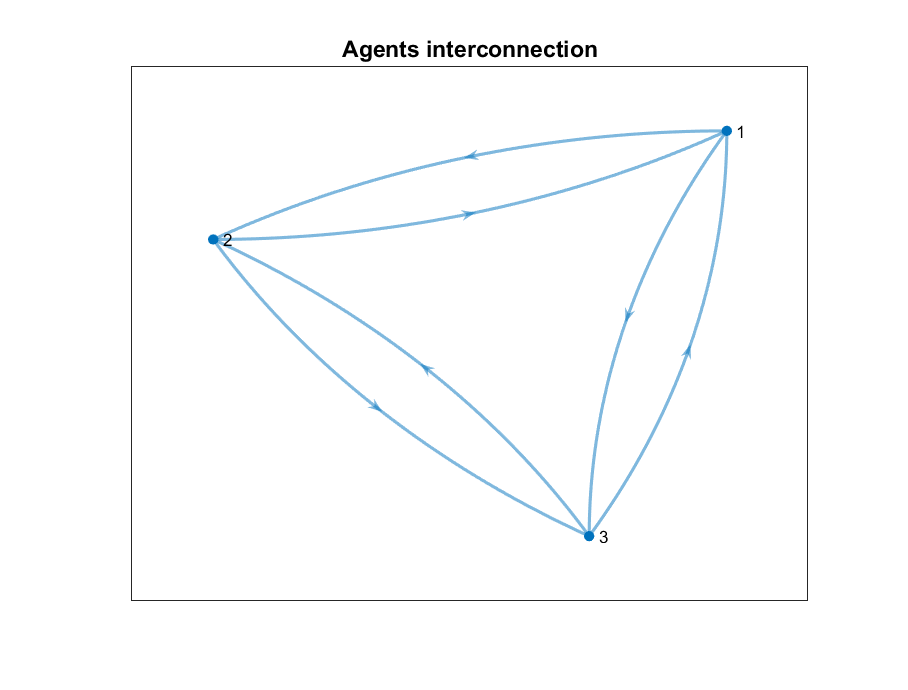
\includegraphics[width=.6\textwidth]{Images/3Agents/Graph.eps}
\caption{Strongly connected and balanced graph for three agents}
\label{Graph3}
\end{figure}

The graph is strongly connected and balanced and every agent exchanges information with the other ones, i.e. the edges are bidirectional. This can also be seen by looking at the second eigenvalue of the Laplacian Matrix which in our case is equal to $\lambda_2 = 6$. We know that the bigger this value is the more connected is the graph. These conditions are necessary in order to apply the control law defined in the previous section.

The adjacency matrix associated to this graph is 
\begin{equation}
A = 
\begin{bmatrix}
0 & 1 & 1\\
1 & 0 & 1\\
1 & 1 & 0
\end{bmatrix}
\end{equation}
\subsubsection*{Rendezvous Problem}

The initial conditions on the positions of the agents and on their headings have been chosen in a random way. In particular 
\begin{align*}
x_0 &= [-10 \quad 12 \quad 10]^T\\
y_0 &= [12 \quad -12 \quad 8]^T\\
\theta_0 &= [\pi/2 \quad \pi/2 \quad 0]^T
\end{align*}

From Fig. \ref{Pos_3_Rend_NW} it can be seen how the control law manages to solve the problem, however it does not care about what kind of motion the unicycles perform. This fact can be easily seen in Fig. \ref{Head_3_Rend_NW} which shows the behaviour of the angle $\theta$. This behaviour is directly related to the control effort which is needed to perform the corresponding motion as shown in Fig. \ref{Contr_3_Rend_NW}. In fact all the variations present in the control $\omega_i$ are reflected in the oscillatory behaviour of the headings of the robots.

\begin{figure}[H]
\centering
\subfloat[][\emph{Positions of the three agents during rendezvous} \label{Pos_3_Rend_NW}]
	{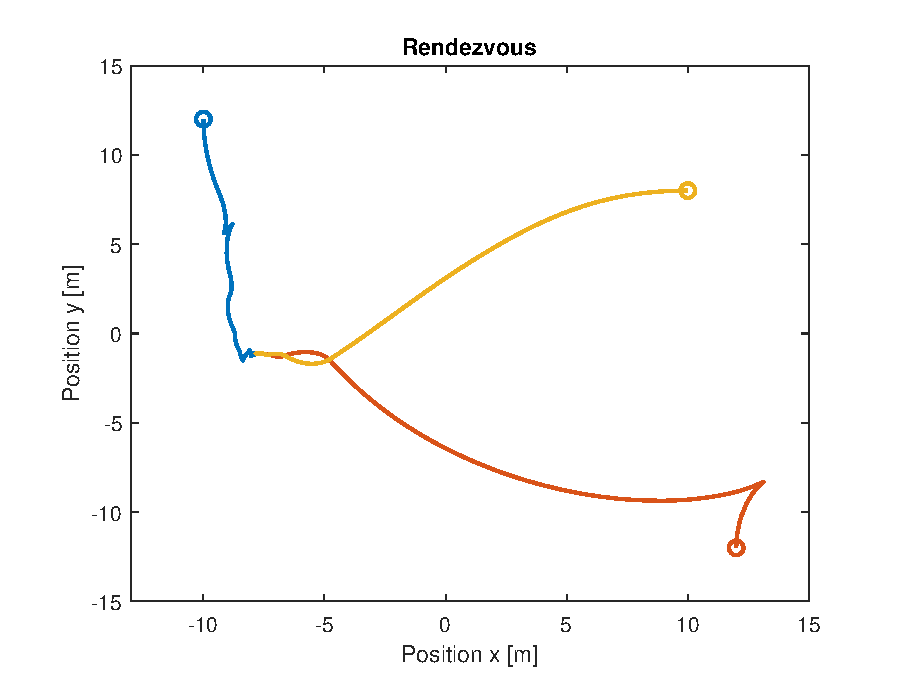
\includegraphics[width=.45\textwidth]{Images/3Agents/Position_Rendezvous_NoWeight.eps}} \quad
\subfloat[][\emph{Headings of the three agents during rendezvous} \label{Head_3_Rend_NW}]
	{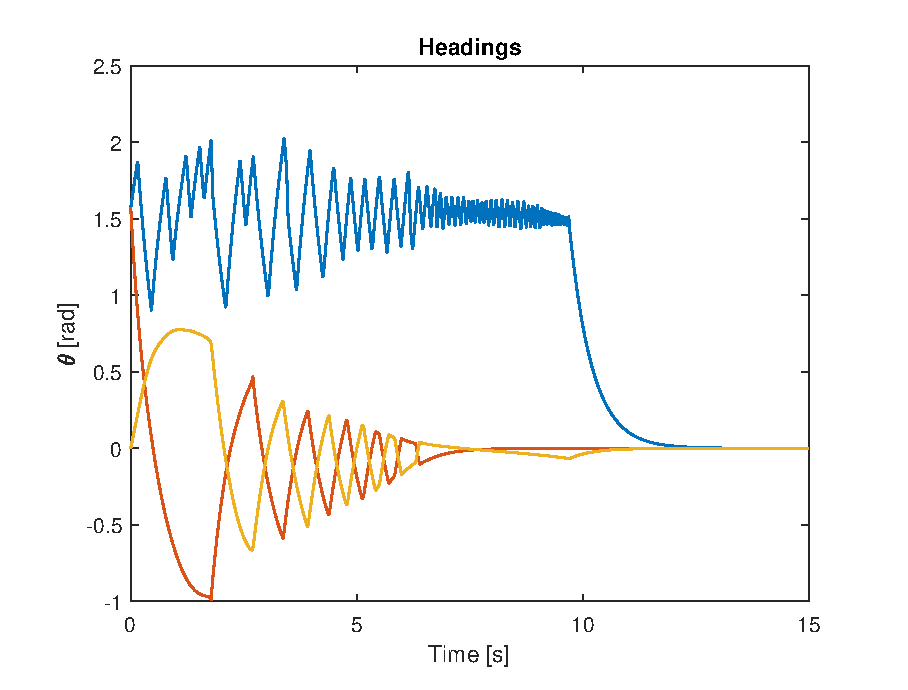
\includegraphics[width=.45\textwidth]{Images/3Agents/Headings_Rendezvous_NoWeight.eps}} 
\caption{Trajectories of the agents during the rendezvous }
\label{fig: 3_Rend_NW}
\end{figure}

On the rendezvous problem has been performed another set of simulations in which the control effort has been weighted by a constant value $k = 0.1$ (Fig. \ref{Contr_3_Rend_W}). This kind of experiment has been done in order to see if, by reducing the control effort, it is possible to improve the previous behaviour. \\
In Fig. \ref{Pos_3_Rend_W} it can be seen how the position trajectories are smoother w.r.t. the previous ones, however the behaviour of the headings is exactly the same except for the fact that it takes more time to reach the desiderd orientation.

\begin{figure}[H]
\centering
\subfloat[][\emph{Positions of the three agents during rendezvous} \label{Pos_3_Rend_W}]
	{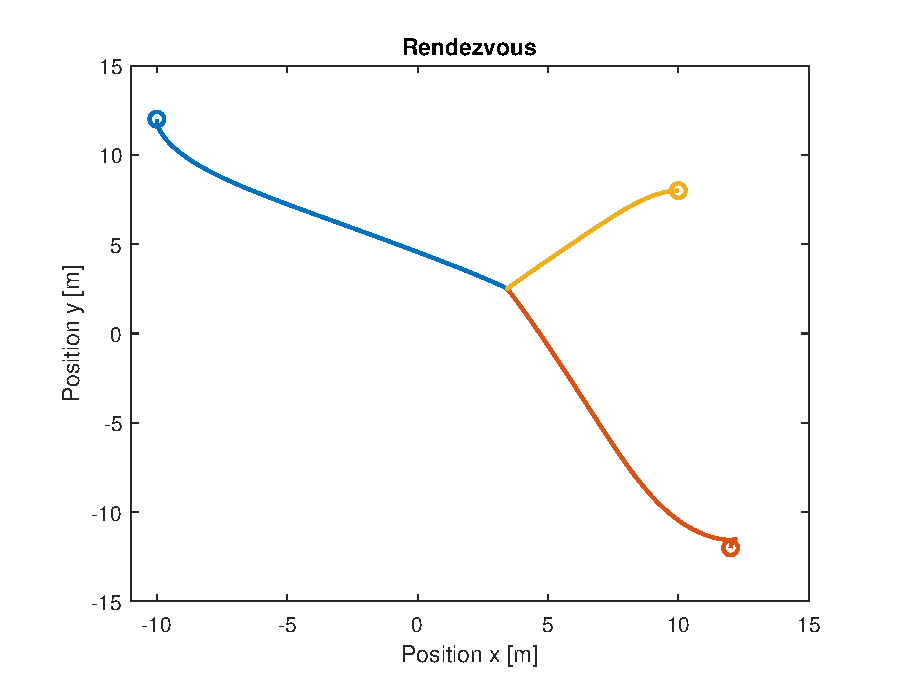
\includegraphics[width=.45\textwidth]{Images/3Agents/Position_Rendezvous_Weight.eps}} \quad
\subfloat[][\emph{Headings of the three agents during rendezvous} \label{Head_3_Rend_W}]
	{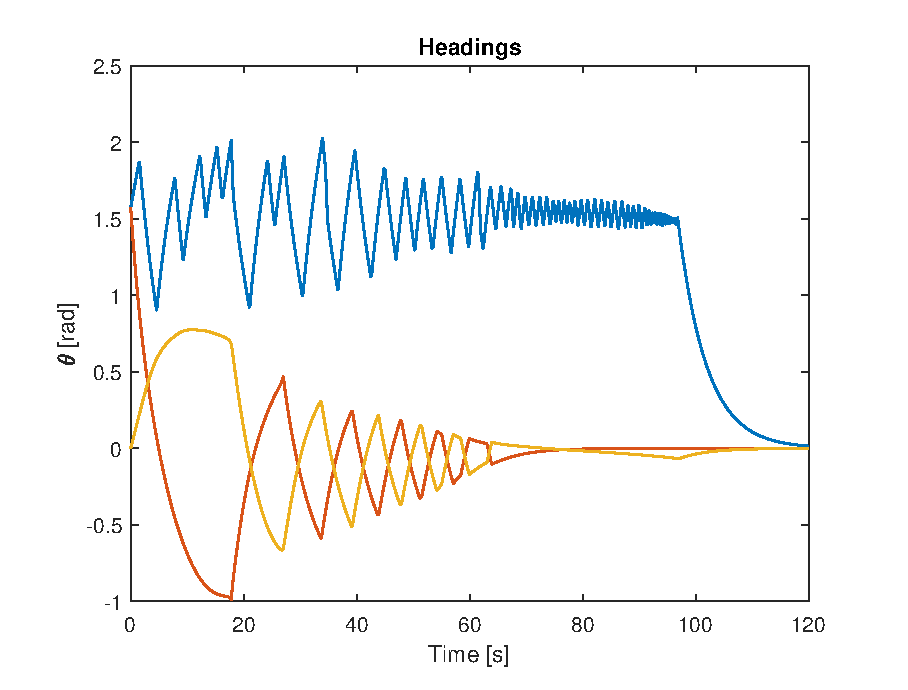
\includegraphics[width=.45\textwidth]{Images/3Agents/Headings_Rendezvous_Weight.eps}} 
\caption{Trajectories of the agents during the rendezvous with a weighted Control Effort}
\label{fig: 3_Rend_W}
\end{figure}

\begin{figure}[H]
\centering
\subfloat[][\emph{Control Effort of the three agents during rendezvous} \label{Contr_3_Rend_NW}]
	{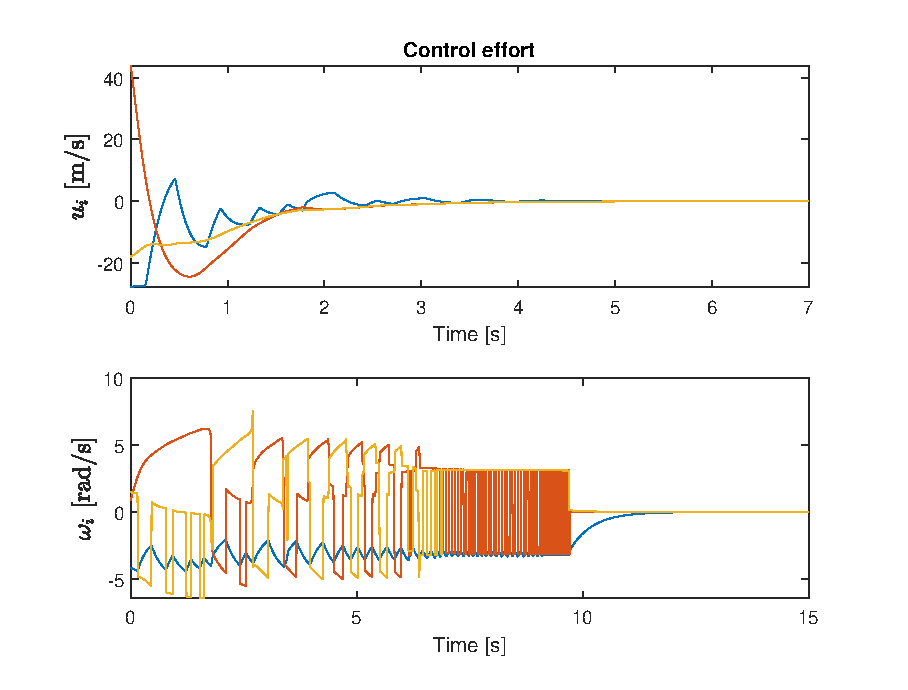
\includegraphics[width=.45\textwidth]{Images/3Agents/Control_Rendezvous_NoWeight.eps}} \quad
\subfloat[][\emph{Weighted Control Effort of the three agents during rendezvous} \label{Contr_3_Rend_W}]
	{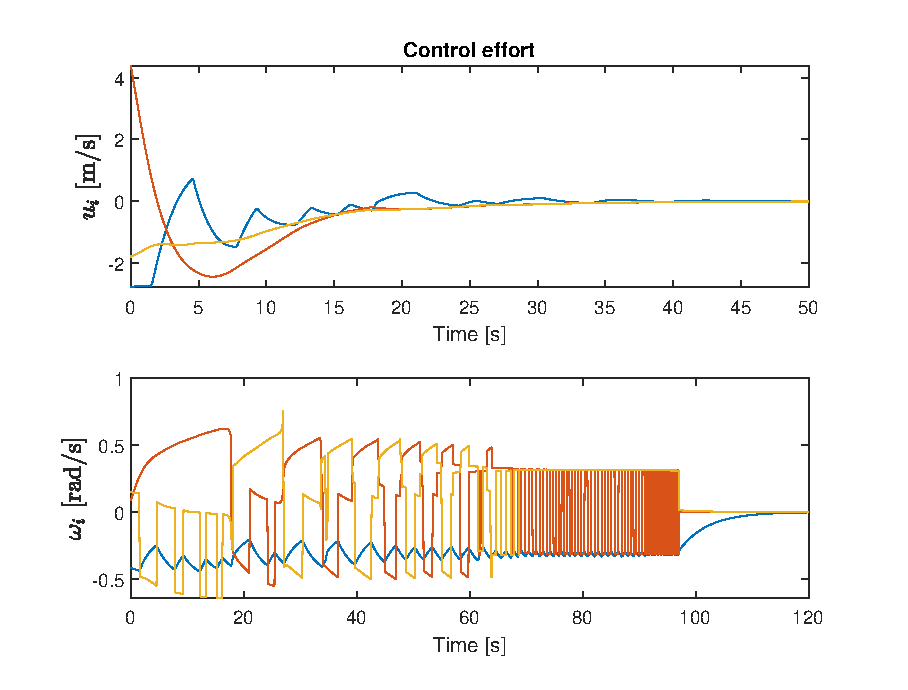
\includegraphics[width=.45\textwidth]{Images/3Agents/Control_Rendezvous_Weight.eps}} 
\caption{Control Effort for the rendezvous problem with and without a weight}
\label{fig: Contr_3_Rend}
\end{figure}


\subsubsection*{Formation Control Problem}

The initial configuration for the three agents is the same as the one used in the rendezvous problem. In particular it has been chosen $\theta_d = 0$, $u_d = 0$, $d = \sqrt{c} = 7$ [m]. This means that, at steady--state, the agents will have to mantain a distance equal to $d$ meters between them with a desired orientation $\theta_d$ and a desired velocity $u_d$. The results can be seen in Fig. \ref{fig: Traj_3_Form}. In Fig. \ref{Pos_3_Form} it can be seen how the agents try to rendezvous in a single point but, when their relative distance reaches the desired value $d$, they stop having the desired orientation. The latter is shown in Fig. \ref{Head_3_Form}. In Fig. \ref{Contr_3_Form} is shown the control effort. Again, due to the nature of the control law, the action does not care about the transient motion as we can see in the behaviour of the angles $\theta_i$.
\begin{figure}[H]
\centering
\subfloat[][\emph{Position of the three agents during Formation Control} \label{Pos_3_Form}]
	{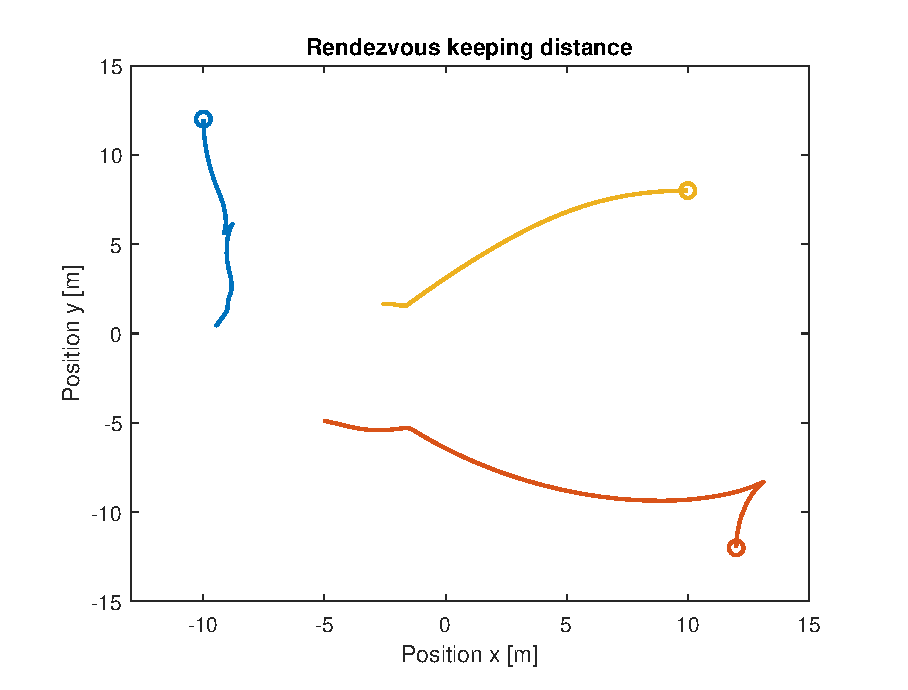
\includegraphics[width=.45\textwidth]{Images/3Agents/Position_Rendezvous_Keeping_Distance.eps}} \quad
\subfloat[][\emph{Headings of the three agents during Formation Control} \label{Head_3_Form}]
	{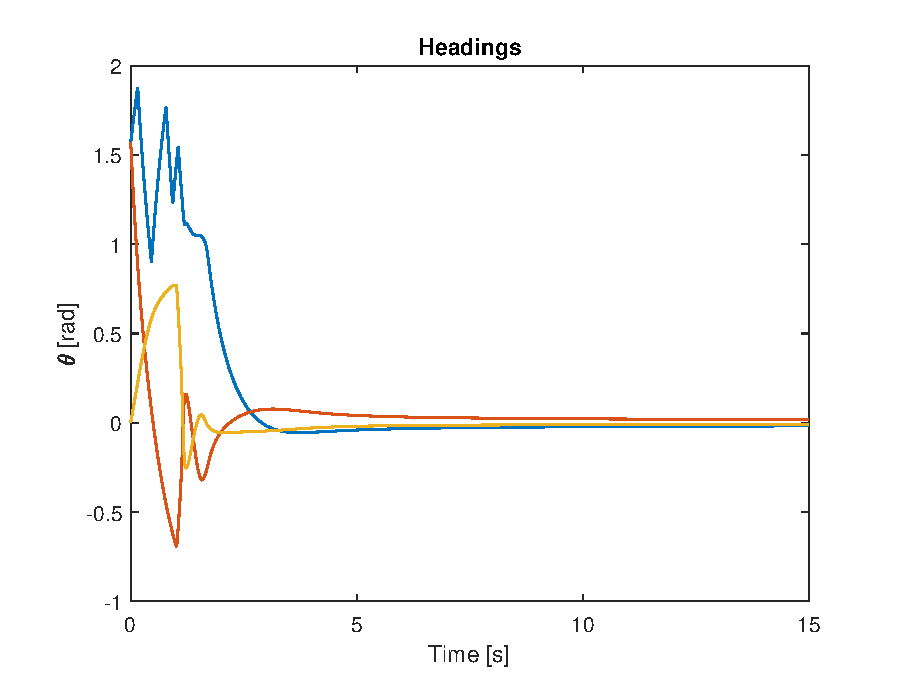
\includegraphics[width=.45\textwidth]{Images/3Agents/Headings_Rendezvous_Keeping_Distance.eps}} 
\caption{Trajectories for the Formation Control problem}
\label{fig: Traj_3_Form}
\end{figure}

\begin{figure}[H]
\centering
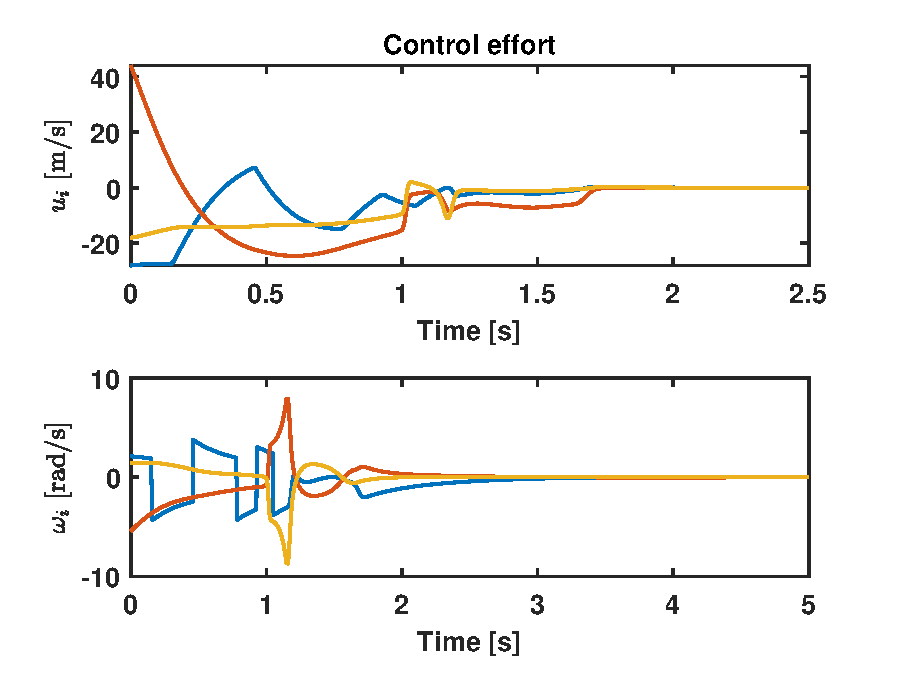
\includegraphics[width=.6\textwidth]{Images/3Agents/Control_Rendezvous_Keeping_Distance.eps}
\caption{Control Effort for the Formation Control}
\label{Contr_3_Form}
\end{figure}

\subsection*{4 agents}

The previous results, obtained for a group of three agents, have been extended to more general cases, in order to evaluate the performance of the control law when the number of unicycles increases.

In the case of four agents, the graph has been modified, maintaining the properties needed to apply the control law. In this scenario, each agent communicates only with one other agent, so it is expected that two agents which do not communicate one with each other will not keep the desired distance in the formation control. The adjacency matrix is
\[
A =
\begin{bmatrix}
0 & 0 & 1 & 0 \\
0 & 0 & 0 & 1 \\
0 & 1 & 0 & 0 \\
1 & 0 & 0 & 0 
\end{bmatrix}.
\]
The graph structure is depicted in Fig.~\ref{graph_4}.

\begin{figure}[H]
\centering
\includegraphics[width=.6\textwidth]{Images/4agents/Graph}
\caption{Graph structure for a multi--robot systems composed by four agents. Note how the couples $(1,2)$ and $(3,4)$ do not have the possibility to communicate.}
\label{graph_4}
\end{figure}

The initial conditions are 
\[
\begin{split}
x_0 & = [-10 \quad 12 \quad 10 \quad -1]^T \\
y_0 & = [12 \quad -12 \quad 8 \quad -15]^T \\ 
\theta_0 & = [\pi/2 \quad -\pi/2 \quad 2\pi/3 \quad \pi]^T.
\end{split}
\]
The rendezvous trajectory in the plane is reported in Fig.~\ref{pos_rendez_4}. The robots, with the proposed control law, are able to perform the rendezvous.

\begin{figure}[H]
\centering
\includegraphics[width=.6\textwidth]{Images/4agents/Position_Rendezvous}
\caption{Position of the four unicycles during rendezvous.}
\label{pos_rendez_4}
\end{figure}

In this case study, the formation control has been implemented imposing a distance $d = \sqrt{c} = 12$ [m], $u_d = 0.9$ [m/s] and $\theta_d = \pi/4$ [rad]. It means that the goal is to perform a rendezvous keeping a distance of 12 [m] between the robots which are able to communicate, and then to start traveling at 0.9 [m/s] in the north--east direction.

The results are shown in Fig.~\ref{results_formation_4}. It is possible to see that the transient which affects the evolution of the headings is very fast ($\approx 4$ [s]): this is due to the fact that the control law has been implemented without using a weight. On the other hand, the robots are able to keep the distance between them (note how the distance between the first robot (blue) and the second one (red) is much larger than 12 [m]: this is coherent with the graph structure defined above). Moreover, it is worth noting that the group of agents keeps the desired orientation for the whole duration of the travel. 

\begin{figure}[H]
\centering
\subfloat[][\emph{Position}]
{\includegraphics[width=.45\textwidth]{Images/4agents/Position_Formation}} \quad
\subfloat[][\emph{Headings}]
{\includegraphics[width=.45\textwidth]{Images/4agents/Headings_Formation}} \\
\caption{Formation control of the four unicycles}
\label{results_formation_4}
\end{figure} 

\subsection*{5 agents}

The last case study is the one with five agents. The network graph is similar to the one defined for the previous case: each robot communicates only with another one. The adjacency matrix is

\[
A =
\begin{bmatrix}
0 & 1 & 0 & 0 & 0 \\
0 & 0 & 1 & 0 & 0 \\
0 & 0 & 0 & 1 & 0 \\
0 & 0 & 0 & 0 & 1 \\
1 & 0 & 0 & 0 & 0 
\end{bmatrix}.
\]
 
The representation of the interconnection is depicted in Fig.~\ref{graph_5}. Note that each unicycle cannot send to nor receive information from two unicycles in the group.

\begin{figure}[H]
\centering
\includegraphics[width=.6\textwidth]{Images/5agents/Graph}
\caption{Graph structure for a multi--robot systems composed by five agents}
\label{graph_5}
\end{figure}

This case study is very interesting because the trajectories that the unicycles have to follow in order to perform the rendezvous are really unrealistic and possible only in the simulation. With five agents, it is possible to appreciate the main property of the control law, which does not take into account the path followed by the players, nor the control effort needed to execute the rendezvous. In few words, the rendezvous is always possible, but it may happen that the trajectories are prohibitive and the control is not realizable by the actuators. 

The initial conditions are 
\[
\begin{split}
x_0 & = [-10 \quad 12 \quad 10 \quad -1 \quad 0]^T \\
y_0 & = [12 \quad -12 \quad 8 \quad -15 \quad 0]^T \\ 
\theta_0 & = [\pi/2 \quad -\pi/2 \quad 2\pi/3 \quad \pi \quad \pi/3]^T.
\end{split}
\]

On Fig.~\ref{pos_rendez_5} it is shown the position of the five agents during the rendezvous operation. The movement is really chaotic and the agents collide one with each other many times during the transient. In any case, the rendezvous problem is still achieved at the end of the simulation.

\begin{figure}[H]
\centering
\includegraphics[width=.6\textwidth]{Images/5agents/Position_Rendezvous}
\caption{Position of the five unicycles during rendezvous.}
\label{pos_rendez_5}
\end{figure}

Regarding the formation control, it is possible to reach the desired motion while keeping the distance between the linked robot, without collision. In order to exploit the power of the proposed control law for the formation, the final constant references have been modified in order to execute an elliptic path.  In formulas
\[
\theta_d = \dfrac{t}{7} \, \textup{[rad]}; \quad u_{x,d} = 3.8 \, \textup{[m/s]}; \quad u_{y,d} = 0.8 \, \textup{[m/s]};.
\]

The results are shown in Fig.~\ref{results_formation_5}. It is possible to appreciate the fact that the robots meet at a certain point keeping an imposed distance $d =$ 5 [m], and then they start traveling along the elliptic path, so increasing their headings as time increases. This result is very powerful, because it shows that with this control law is possible to execute a user--defined random path by ensuring the distance between the agents.

\begin{figure}[H]
\centering
\subfloat[][\emph{Position}]
{\includegraphics[width=.45\textwidth]{Images/5agents/Position_Formation}} \quad
\subfloat[][\emph{Headings}]
{\includegraphics[width=.45\textwidth]{Images/5agents/Headings_Formation}} \\
\caption{Formation control of the five unicycles}
\label{results_formation_5}
\end{figure}



%Codice per inserire il codice
\begin{comment}
\singlespacing
\begin{Verbatim}[tabsize = 4, frame = lines, numbers = left]
code_here...
	code_here...
code_here...
\end{Verbatim}
\onehalfspacing
\end{comment}

\begin{thebibliography}{2}

	\bibitem{listmann}
	Listmann K. D., Masalawala M. V. and Adamy J., (2009), \textit{Consensus for Formation Control of 			Nonholonomic Mobile Robots}, IEEE International Conference on Robotics and Automation, Kobe, Japan, 		pp. 3896--3891.
	
	\bibitem{cristofaro}
	Cristofaro A., (2020), \textit{Control of Multi--Robot Systems}, Lecture Notes.


\end{thebibliography}
\end{document}
